\documentclass{beamer}

\usepackage{lmodern}
\usepackage[english]{babel}
\usepackage[utf8]{inputenc}
\usepackage{amsmath, amsthm}
\usepackage{amsfonts}
\usepackage{mathtools}
\usepackage{graphicx}
\usepackage[colorinlistoftodos]{todonotes}
\usepackage[affil-it]{authblk}
\usepackage[parfill]{parskip}
\usepackage{subfig}
\usepackage{float}

\usetheme{metropolis} % Use metropolis theme

\title{A Guide to Optimization and Optimal Play in Greed}
\author{Chance Addis}
\affil{Department of Mathematics and Statistics, Reed College}

\begin{document}

\maketitle

%% ----- SECTION: ABSTRACT ----- %%
\section{Abstract}

\begin{frame}{Goals}
    The game of Greed is a probabilistic two-player game. The goal of this project is to derive an optimal way to play the game - based on reasonable heuristic metrics - as well as as determine the optimal chance of success, as determined by out heuristic. 
\end{frame}

\begin{frame}
    Why: 

    \begin{itemize}
        \item You will (probably) be really good at Greed.
        \item This project is a good starter problem for learning about reinforcement learning.
    \end{itemize}
\end{frame}

%% ----- SECTION: HOW DO YOU PLAY GREED AGAIN ----- %%
\section{How Do You Play Greed Again?}
\begin{frame}{Game Environment \& Turns}
    Greed is a game that could be described as ``kinda like blackjack with dice''.

    \textbf{Game parameters:}
    
    $M$: max score before going bust. \\
    $s$: number of sides on each die.

    \textbf{Starts at}
    $s_p = 0$ and $s_o = 0$ respectively.

    Each turn, the player up to roll will choose some $n \in \mathbb{N}^0$ number of dice to roll. Then the sum of those dice will be added to their score. Players will go back and forth like this until one of two terminal states is reached.
\end{frame}

\begin{frame}{How To Win}
    \begin{enumerate}
        \item In the first option, a player's score goes over $M$, i.e. and they go bust. In this case, they lose, so we'll say that their rating -- the heuristic measure that we use to measure how good a position is -- is 0, and thus their opponents rating is 1. 
        \item In the second option, a player can choose to roll 0 dice. This will initiate the last turn. The other player will then have one more chance to roll. The winner is the player who has the higher score that is not over $M$. In the case of a tie, rating is 1/2 for each player. 
    \end{enumerate}
\end{frame}

%% ----- SECTION: MATHEMATICAL FRAMEWORK ----- %%
\section{Mathematical Framework}
\begin{frame}{Mathematical Framework}
    Consider two types of states: terminal states, which denote the last turn of the game, and normal turns, representing all other states. 

    Normal and terminal states are conceptualized as 2 by 2 arrays with dimension $M+1$ by $M+1$, representing all possible states for player and opponent.
    
    The x-axis designates the player presently up to roll, while the y-axis designates the player who has just rolled.

    Therefore, any state $S$ can be defined by the tuple $(s_0, s_1, l)$
\end{frame}

%% ----- SECTION: PMF ----- %%
\section{PMF, PMF, PMF}
\begin{frame}{What Is The Random Variable}
    First, consider just a single dice. It has pmf
    %
    $$
    D_{i}^{(s)}(d) = \begin{cases}
        \frac{1}{s} & \text{if } d \in \{1, \ldots, s \} \\
        0 & \text{otherwise}
    \end{cases}
    $$
    %
    So let the random variable $T$ denote the sum of $n$ iid random dice, each with $s$ sides. It can thusly be written
    %
    $$ 
    T: \left(\mathbb{N}_{0}\right)^n \to \mathbb{R}, T \coloneqq D_{1}^{(s)}(d_1) + \cdots + D_{n}^{(s)}(d_n) 
    $$
    %
    Therefore, our goal is to find the pmf of $T$, which is notated $\textbf{p}_{T}^{(n, s)}(t)$, dependent on parameters $n, s$. 
\end{frame}

\begin{frame}{Moment-Generating Functions}
    In order to find the probability mass function of $T$, we'll use moment generating functions. Remember that probability distributions and moment generating functions have a one-to-one correspondence. So for a discrete random variable $X$ with probability distribution
    %
    $$ 
    f(x_i) = P(X = x_i) = p_i \text{ for } i = 1, 2, \ldots k 
    $$
    %
    then it's mfg is
    %
    \begin{align*}
        M_X(t) &= \mathbb{E}[e^{tX}] = \sum_{x} e^{tx} \cdot f(x) =  \\ 
        &= p_1 \cdot e^{tx_1} + p_2 \cdot e^{tx_2} + \cdots + p_k \cdot e^{tx_k}.
    \end{align*}
    %
    and visa verse (like in [\textit{HW 6, 2.1}]).

    So for $t = 1$, $P(X = x)$ is the coefficient of $e^x$. 
\end{frame}

\begin{frame}{What is the moment generating function of $T$?}
    Recall the pmf of $D_{i}^{(s)}$. It's moment generating function is defined as
    %
    $$
    M_{D_{i}^{(s)}}(t) = \mathbb{E}[e^{tD_{i}^{(s)}}] = \frac{1}{s}(e^{t} + e^{2t} + \cdots + e^{st})
    $$
    %
    Since $D_{i}^{(s)}$ are all independent and identically distributed,
    %
    \begin{align*}
        M_{T}(t) &= \mathbb{E}[e^{tT}] = \mathbb{E}[e^{t(D_{1}^{(s)} + \cdots + D_{n}^{(s)})}] = \prod_{i = 1}^{n} \mathbb{E}[e^{tD_{i}^{(s)}}] \\
        &= \prod_{i = 1}^{n} \left[\frac{1}{s}(e^{t} + e^{2t} + \cdots + e^{st}) \right] \\
        &= \frac{1}{s^n} (e^{t} + e^{2t} + \cdots + e^{st})^n
    \end{align*}
\end{frame}


\begin{frame}{Formula for Coefficients of the Mulitnomials (Strap In)}
    Skipping over the complex algebra, the coefficient $x^t$ in the expanded multinomial are found with
    %
    $$
    \frac{1}{s^n} \sum_{k = 0}^{\lfloor\frac{t-n}{s} \rfloor} (-1)^k \binom{n}{k} \binom{t-sk-1}{n-1}
    $$ 

    And as explained, these coefficients map to the probabilities of the pmf, so the pmf of $T$ is written
    %
    $$
    \textbf{p}_{T}^{(n, s)}(t) = \frac{1}{s^n} \sum_{k = 0}^{\lfloor\frac{t-n}{s} \rfloor} (-1)^k \binom{n}{k} \binom{t - s \cdot k - 1}{n-1}
    $$
\end{frame}

%% ----- SECTION: OPTIMIZATION OF TERMINAL STATE  ----- %%
\section{Terminal States}

\begin{frame}{Defining a Rating Function on Terminal States}
    The goal is to find some $n$ to maximize the probability of getting a new score $s_p + t$ between $s_o$, and $M$?" 
    
    Or more precisely, given a state $(s_p, s_o, 1)$, what is the optimal $n$ such that the expected rating is maximized.  
    %
    \begin{align*}
        \text{rating}((s_p, s_o, 1), n) \coloneqq \sum_{t = s_o+1}^{\text{M}} \textbf{p}_{T}^{(n, s)}(t - s_p) + \frac{1}{2} \cdot \textbf{p}_{T}^{(n, s)}(s_o - s_p)
    \end{align*}
    %
    where the summation describes the weighted sum of all next states given $n$, weighted according to their probability (transition matrix), hence rating is the expectation of its next possible states. 
\end{frame}

\begin{frame}{Optimal Actions and Ratings on Terminal States}
    Since $n_{\star}$ is the optimizer of rating, it is given by
    %
    \begin{align*}
        n_{\star}(s_0, s_1, 1) \coloneqq \text{argmax}_n \left\{ \text{rating}((s_0, s_1, 1), n) \right\}
    \end{align*}
    %
    Notice that the optimal rating comes for free. It's the rating that was optimized for in finding $n_{\star}$, so no additional work is required.
    %
    \begin{align*}
        \text{rating}_{\star}((s_p, s_o, 1), n_{\star}) \coloneqq \text{rating}((s_p, s_o, 1), n_{\star})
    \end{align*}
\end{frame}

%% ----- SECTION: OPTIMIZING NORMAL STATES ----- %%
\section{Optimizing Normal States}

\begin{frame}{Defining a Rating Function on Normal States}
    The rating is defined in the same way as it is for terminal states: The expectation of the rating for the next possible states $S_1$ given some $n$. 

    \textbf{Example}

    Let's give an example. Imagine that the optimal $n_{\star}$ and $\text{rating}_{\star}$ for every other state is known. 

    Consider rolling $2$ dice at state $(2, 6)$. You could end up at any of the following states: $S_1 = \{(6, 4), (6,5), (6,6), (6,7)\}$. So since we know the rating of all these states, we can calculate the rating given $n$ by taking the weighted sum over $S_1$, with weights given by the pmf of $T$, i.e. $\textbf{p}_{T}^{(n, s)}(2), \ldots, \textbf{p}_{T}^{(n, s)}(4)$.
\end{frame}

\begin{frame}{Defining a Rating Function on Normal States}
    \textbf{Fact:} Rating is complementary with respect to each player's rating for a given state.

    Hence, the optimal rating for landing on a state $S$ is $1-\text{rating}(S, n_{\star})$ (since the rating of that state will be for the opponent), where $n_{\star}$ is the optimal $n$ for that state. 


    So the rating function is given by
    %
    \begin{align*}
        \text{rating}(S, n) \coloneqq \begin{cases}
            \sum_{t = n}^{s \cdot n} 1 - \text{rating}((s_o, s_p + t, 0), n_{\star}) & \text{if } n > 0 \\
            1- \text{rating}((s_o, s_p, 1), n_{\star}) & \text{if } n = 0
        \end{cases}
    \end{align*}
\end{frame}

\begin{frame}{Optimal Actions and Ratings on Normal States}
    Thus the optimal $n_{\star}$ given any possible state $S$, normal or terminal is now defined to be
    %
    $$
    n_{\star} = \text{argmax}_{n} \left\{\sum_{t = n}^{s \cdot n} 1 - \text{rating}((s_o, s_p + t, \{0 \text{ if } n = 1 \text{ else } 0\}) \right\}
    $$
    %
    where the rating function could be the one defined for terminal states or normal states.

    $\text{rating}_{\star}$ is defined the same as for terminal states.
\end{frame}

%% ----- SECTION: RESULTS ----- %%
\section{Cool Plots}

\begin{frame}{Terminal States Results}
    \begin{figure}[h]
        \centering
        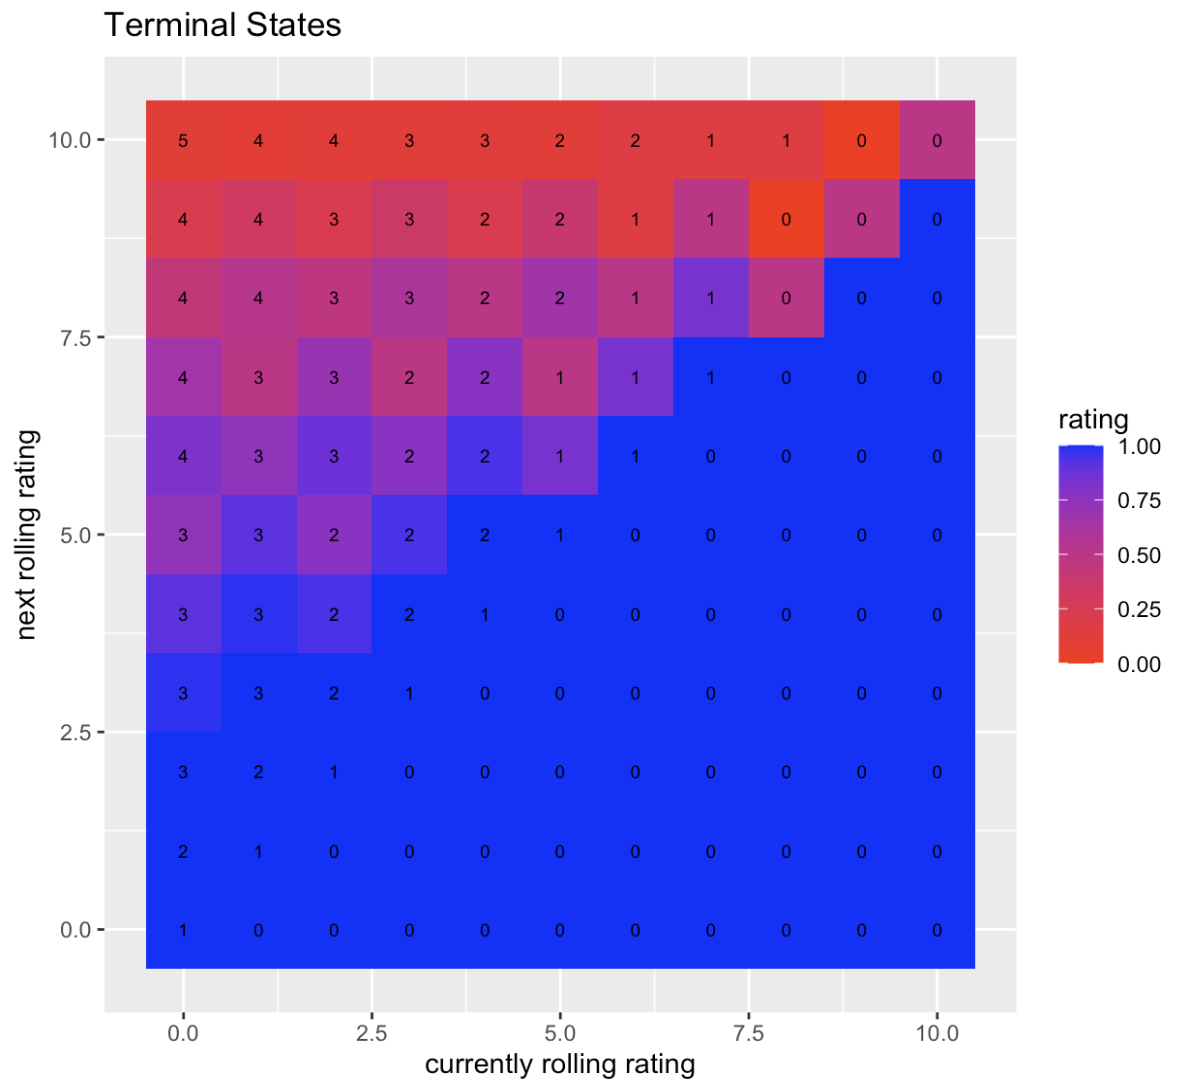
\includegraphics[width=0.7\textwidth]{Screenshot 2023-12-12 at 20.21.12.png}
        \caption{Optimal Actions and Ratings for Terminal States}
    \end{figure}
\end{frame}

\begin{frame}{Normal States Results}
    \begin{figure}[h]
        \centering
        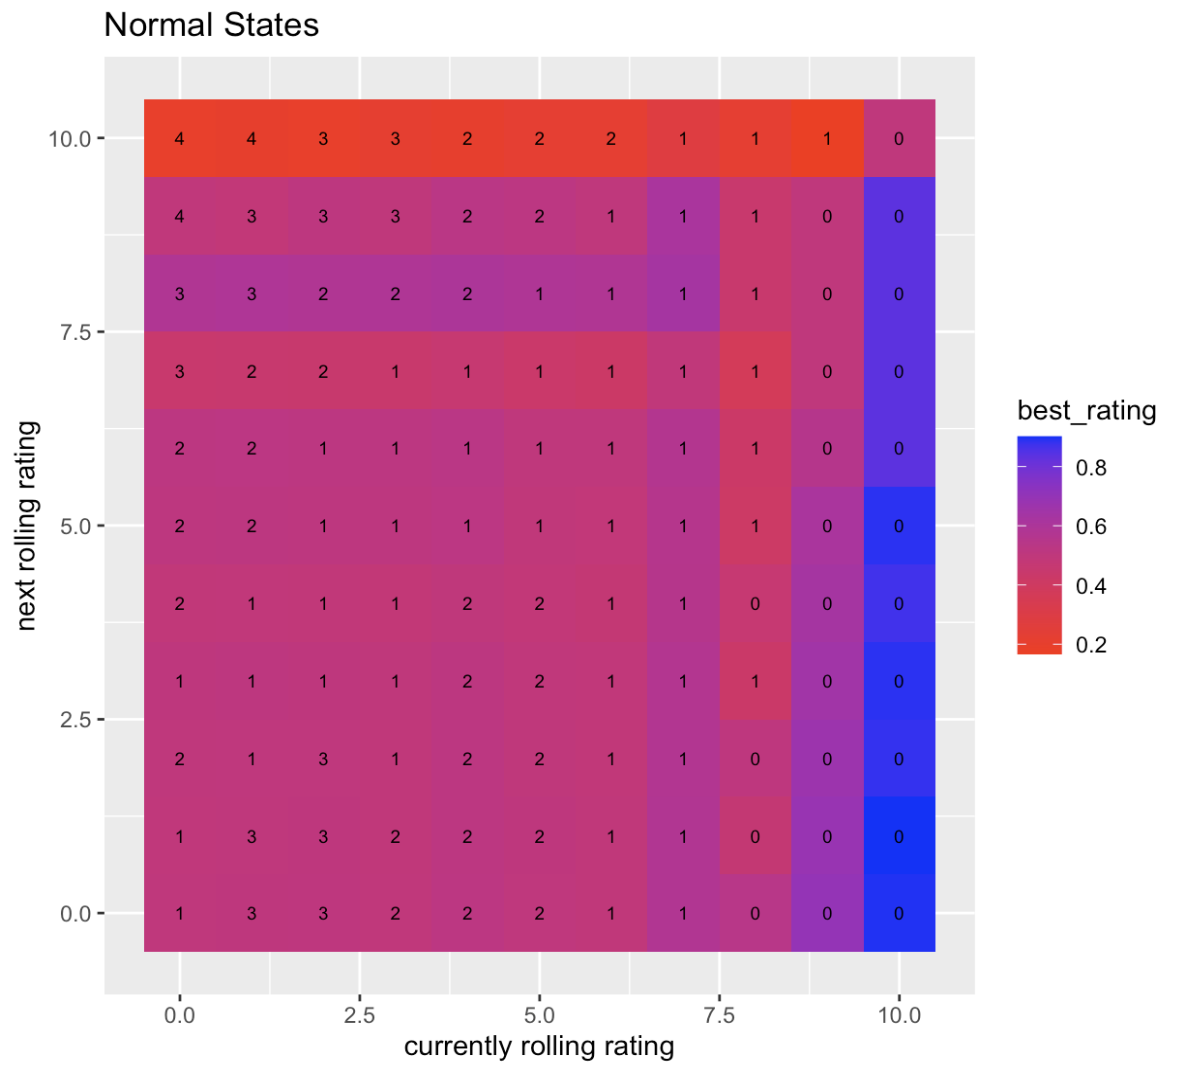
\includegraphics[width=0.7\textwidth]{Screenshot 2023-12-14 at 01.43.15.png}
        \caption{Optimal Actions and Ratings for Normal States}
    \end{figure}
\end{frame}

%% ----- SECTION: CONCLUSION ----- %%
\section{Conclusion}

\begin{frame}{Important Results}
    \begin{itemize}{}
        \item Found a metric for determining success in Greed
        \item Found the pmf of $n$ independent and identically distributed discrete uniform random variables, each with $s$ outcomes. 
        \item Found a rating function for all possible states that could occur in Greed.
        \item Found a optimal move and rating for every possible state in Greed
    \end{itemize}
\end{frame}

\begin{frame}{Limitations}
    \begin{itemize}{}
        \item Rating is not an objective measurement
        \item The way that states rely on each other may not be optimal
        \item The code that runs the calculations could still have many bugs and possible edge cases (I would like to concur on the possibility of this outcome).
    \end{itemize}
\end{frame}

\begin{frame}{Additional Research}
    \begin{itemize}{}
        \item A more mathematically rigorous mathematical framework.
        \item Determin whether there some pattern on normal states that can allow us to infer their rating more easily.
        \item etc
    \end{itemize}
\end{frame}

\begin{frame}{Stuff That Got Left Out}
    \begin{itemize}{}
        \item Calculations for getting the coefficient of the multinomial
        \item Algorithm for finding the optimal n and rating for terminal states.
        \item Algorithm for finding the optimal n and rating for normal states.
    \end{itemize}
\end{frame}

\end{document}
